%%%%%%%%%%%%%%%%%%%%%%% file template.tex %%%%%%%%%%%%%%%%%%%%%%%%%
%
% This is a general template file for the LaTeX package SVJour3
% for Springer journals.          Springer Heidelberg 2010/09/16
%
% Copy it to a new file with a new name and use it as the basis
% for your article. Delete % signs as needed.
%
% This template includes a few options for different layouts and
% content for various journals. Please consult a previous issue of
% your journal as needed.
%
%%%%%%%%%%%%%%%%%%%%%%%%%%%%%%%%%%%%%%%%%%%%%%%%%%%%%%%%%%%%%%%%%%%
%
% First comes an example EPS file -- just ignore it and
% proceed on the \documentclass line
% your LaTeX will extract the file if required
\begin{filecontents*}{example.eps}
%!PS-Adobe-3.0 EPSF-3.0
%%BoundingBox: 19 19 221 221
%%CreationDate: Mon Sep 29 1997
%%Creator: programmed by hand (JK)
%%EndComments
gsave
newpath
  20 20 moveto
  20 220 lineto
  220 220 lineto
  220 20 lineto
closepath
2 setlinewidth
gsave
  .4 setgray fill
grestore
stroke
grestore
\end{filecontents*}
%
\RequirePackage{fix-cm}
%
%\documentclass{svjour3}                     % onecolumn (standard format)
%\documentclass[smallcondensed]{svjour3}     % onecolumn (ditto)
\documentclass[smallextended]{svjour3}       % onecolumn (second format)
%\documentclass[twocolumn]{svjour3}          % twocolumn
%
\smartqed  % flush right qed marks, e.g. at end of proof
%
\usepackage{graphicx}
%
% \usepackage{mathptmx}      % use Times fonts if available on your TeX system
%
% insert here the call for the packages your document requires
%\usepackage{latexsym}
% etc.
%
% please place your own definitions here and don't use \def but
% \newcommand{}{}
%
% Insert the name of "your journal" with
% \journalname{myjournal}
%
\begin{document}

\title{Lactamotion:%\thanks{Grants or other notes
%about the article that should go on the front page should be
%placed here. General acknowledgments should be placed at the end of the article.}
}
\subtitle{Postpartum mobility in northwestern Namibia}

%\titlerunning{Short form of title}        % if too long for running head

\author{Layne Vashro
}

%\authorrunning{Short form of author list} % if too long for running head

\institute{L. Vashro \at
              270 South 1400 East, Salt Lake City, UT 84112 \\
              Tel.: +001 (801) 581 6251\\
              \email{layne.vashro@anthro.utah.edu}           %  \\
}

\date{Received: date / Accepted: date}
% The correct dates will be entered by the editor


\maketitle

\begin{abstract}
Insert your abstract here. Include keywords, PACS and mathematical
subject classification numbers as needed.
\keywords{First keyword \and Second keyword \and More}
% \PACS{PACS code1 \and PACS code2 \and more}
% \subclass{MSC code1 \and MSC code2 \and more}
\end{abstract}

\section{Introduction}
\label{sec:1}
Researchers consistently find sex-differences in spatial-cognitive and navigational tasks, as well as measures of geographical range of movement.  These differences are well-documented in Western industrialized societies and have increasingly been replicated cross-culturally.  Psychologists have proposed several different theories linking these sex differences into a cohesive evolutionary story.  Ancestral males who traveled more safely and effectively long-distance and into unfamiliar terrain in search of mates, game, or batter (cite, cite, cite) were paid in fitness.  This selected for superior navigation ability and the underlying spatial-cognitive traits that facilitate navigational performance.  However, not all evolutionary explanations for this cluster of sex differences focuses on adaptive advantages in men.  Sherry and Hampson (cite) are consistent with the other theories, but rather than focus on men looks at the fitness ramifications of women's long-distance mobility.  This ``fertility and parental care hypothesis'' explains the observed sex differences in terms of the potential costs to women traveling, particularly during key period of reproduction.

	\subsection{Fertility and parental care}
	\label{sec:1.1}
The idea of risky males and risk-averse females has been broadly applied in the evolutionary literature.  Discuss Cambell... Mobility especially in the form of travel outside of one's home range, seems a particularly appropriate topic for applying this heuristic.  

Particular issues.  Cambell and ``staying alive''... segue into issues of infanticide and rape...  Caloric expenditure

Mechanism: i.e. mediated by estrogen and probably other stuff.

	\subsection{Post-partum hormones and spatial ability}
	\label{sec:1.2}
Looking across the entire life-cycle, it is true that women's estrogen level rise as they enter reproductive maturity (is this tru?), and fall after menopause.  This lines up with the theory linking decreased mobility as a risk reduction strategy that is mediated by estrogen.  However, looking within women of reproductive age the pattern of estrogen cycles is more difficult to link with at least a simple version of risk reduction.  The problem is that women's estrogen level drop post-partum.  The team between  birth and weaning is likely \emph{the} time when the concerns highlighted by the fertility and parental care hypothesis should be most important. Instead, at least among mice, this period is associated with improved performance in maze tasks ans increased range (nest visits?... check this). 

\section{Methods}
\label{sec:2}
	\subsection{Population}
This study includes all women living in the \emph{Ovizorowe} mountain valley in northwestern Namibia.  This sample includes mostly members of the Twe ethnic group who live in several villages dispersed throughout the valley, as well as women from some Himba and Tjimba communities bookending the valley. 


Text with citations \cite{RefB} and \cite{RefJ}.
	\subsection{Mobility interviews}
	\label{sec:2.1}
Participants were asked to name each place they traveled to and spent the night in the past year.  In addition, they were asked who they traveled with, who they stayed with, and why they made the trip.  These data were used to create two highly-correlated measures of annual range size.  1) The number of unique places visited in the past year, and 2) the number of kilometers needed to visit each place visited in the past year.  In addition, the analysis is able to discriminate between pair, group, and unaccompanied travel, and identify patterning in the function of travel.
 	
	\subsection{Spatial cognition}
	\label{sec:2.2}
This study includes four different measures of spatial cognition: Mental rotation, Corsi blocks, real-world distant pointing accuracy, and a perspective-taking task (check whether performance is good enough to seriously include).

		\subsubsection{Mental rotation}
		\label{sec:2.2.1}		
This task was administered on an N-inch touch-screen computer.  Participants are shown a screen with two cartoon bodies, one with a left and the other with a right hand outstretched and each rotated on a two-dimensional axis.  The participants are also shown a third figure on the (bottom?) oriented perfectly vertical with either a left or right hand outstretched.  The participant is then asked to indicate which of the two rotated bodies is the same as the third.  Performance is measured both in accuracy across N trials and response time.

This task was readily understood by most participants, but not all...		
	
		\subsubsection{Corsi blocks}
		\label{sec:2.2.2}
This task was also administered on an N-inch touch-screen computer.  Participants are shown a screen with N ? colored squares on a black background.  The participant was asked to watch as blocks are highlighted in a set sequence and then asked to touch the same squares in the same order.  The first two iterations required participants to recall a two-block sequence, the next two iterations required participants to recall a three-block sequence... and so on until the participant failed on two consecutive trials. (make sure ``two'' is correct here and it isn't actually three).

Participants had minimal trouble understanding this task.  In several cases, the participant's fingers were too calloused to use the touch screen and instead they indicated for the experimenter to touch on their behalf.  This does not appear to have impacted the results (is this true?)    		
		
		
		\subsubsection{Pointing}
		\label{sec:2.2.3}
The researcher named a distant location and the participants rotated a Brunton compass mounted on a tripod until it indicated the bearing to that location, to the best of their knowledge.  This process was repeated for ten known locations ranging from 10km to 140km (recheck these figures).  In addition to collecting the bearing indicated by participants, the researcher also asked when was the last time the participant had visited each place, and whether they had been there "once", "a few times", or "many" throughout their lives.  For the analysis, participants' bearing was compared to actual bearing based on GPS coordinates from the point-of-origin and targeted locations.   		

Participants were tested at N different locations.  This creates a problem for comparing pointing accuracy because the varying points-of-origin results in a different task for each participant.  In addition, not all participants were comfortable pointing to all of the locations.  Some of the locations had not been visited by all participants, and you cannot point to a location you do not know.  To account for both of these issues, I analyzed the data across each pointing event while treating the individuals as random effects.  This allowed me to estimate a ``distance'' effect, which was then applied to each pointing event to create difficulty-adjusted measures of accuracy that could then by averaged for each individual creating a single measure of each participant's pointing accuracy. 		
			
		\subsubsection{Perspective taking}
		\label{sec:2.2.4}			


\section{Results}
\label{sec:3}
Text with citations \cite{RefB} and \cite{RefJ}.
	\subsection{Mobility interviews}
	\label{sec:3.1}
Your text comes here. Separate text sections with	

% For one-column wide figures use
\begin{figure}[!htb]
  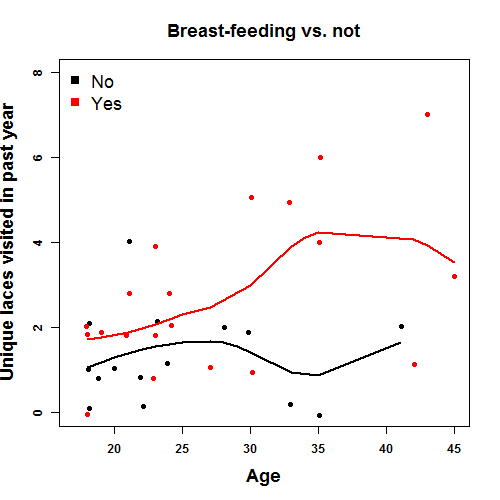
\includegraphics[width=0.75\textwidth]{bfeed_mob}
\caption{Please write your figure caption here}
\label{fig:1}       % Give a unique label
\end{figure}

	\subsection{Spatial cognition}
	\label{sec:3.2}
Your text comes here. Separate text sections with

		\subsubsection{Mental rotation}
		\label{sec:3.2.1}
	
		\subsubsection{Corsi blocks}
		\label{sec:3.2.2}
		
		\subsubsection{Pointing}
		\label{sec:3.2.3}

		\subsubsection{Perspective taking}
		\label{sec:3.2.4}

\section{Discussion}
\label{sec:4}
Comparing reproductive-aged women living in the \emph{Ovizorowe} Valley with and without nursing depends highlights interesting differences in both cognition and mobility.  Breastfeeding women performed better across our measures of spatial cognition (excepting the perspective-taking task), which is consistent with expectations based on the decline in estrogen associated with the post-partum period.  In addition, breastfeeding women were more mobile, traveling to more unique locations and covering more ground in doing so than their peers who were without an unweaned child over that period of time.  This increase in mobility may also be consistent with the down-tick in estrogen and improved spatial cognition from the perspective of several theories linking spatial cognitive ability to distant ranging.  

These findings simultaneously support the patterns of cognition and behavior anticipated by the fertility and parental care hypothesis while complicating the interpretation with the fact that women are most mobile exactly when it seems least likely from the perspective of minimizing risk to offspring.

Why would it be beneficial for women to range further when they have unweaned children?  One study among conducted among a nearby  Himba population (Scelza) showed women traveling the most to visit their mothers during periods of peak childcare need.  This seems an appealing answer to this situation as well, however, most of these women were actually moving \emph{away} from their mothers (is this true??) as a much greater fraction of this population lives matrilocally.  In addition, none of the women explicitly cited visiting their mother.  Several other alternatives... 1) ``Facebook'' effect...  ``Look at the baby, look at the baby''... making connections to relatives who may be called on in future times of need.  2) Rape deterred... then what about pregnancy??  Don't like this.

Interested in future work looking at the volume and function of women's postpartum mobility in other populations, including the US.


Text with citations \cite{RefB} and \cite{RefJ}.

%
% For two-column wide figures use
\begin{figure*}
  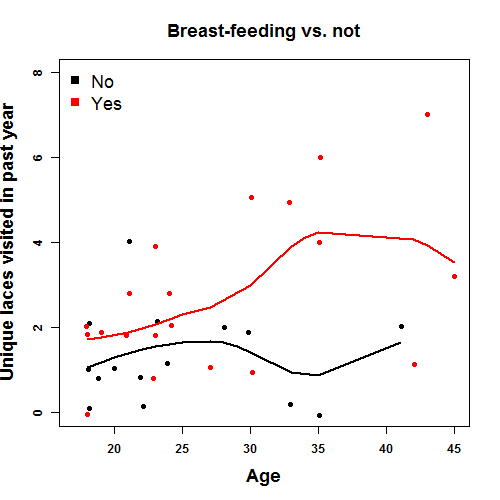
\includegraphics[width=0.75\textwidth]{bfeed_mob}
\caption{Please write your figure caption here}
\label{fig:2}       % Give a unique label
\end{figure*}
%
% For tables use
\begin{table}
% table caption is above the table
\caption{Please write your table caption here}
\label{tab:1}       % Give a unique label
% For LaTeX tables use
\begin{tabular}{lll}
\hline\noalign{\smallskip}
first & second & third  \\
\noalign{\smallskip}\hline\noalign{\smallskip}
number & number & number \\
number & number & number \\
\noalign{\smallskip}\hline
\end{tabular}
\end{table}


%\begin{acknowledgements}
%If you'd like to thank anyone, place your comments here
%and remove the percent signs.
%\end{acknowledgements}

% BibTeX users please use one of
%\bibliographystyle{spbasic}      % basic style, author-year citations
%\bibliographystyle{spmpsci}      % mathematics and physical sciences
%\bibliographystyle{spphys}       % APS-like style for physics
%\bibliography{}   % name your BibTeX data base

% Non-BibTeX users please use
\begin{thebibliography}{}
%
% and use \bibitem to create references. Consult the Instructions
% for authors for reference list style.
%
\bibitem{RefJ}
% Format for Journal Reference
Author, Article title, Journal, Volume, page numbers (year)
% Format for books
\bibitem{RefB}
Author, Book title, page numbers. Publisher, place (year)
% etc
\end{thebibliography}

\end{document}
% end of file template.tex

